\documentclass[final,5p,12pt,twocolumn]{elsaarticle}
\usepackage{minted}
\usepackage{fancyvrb}
\usepackage{amssymb}
\usepackage[a4paper]{geometry}
 \geometry{twoside,
  paperwidth=210mm,
  paperheight=297mm,
  textheight=700pt,
  textwidth=474pt,
  centering,
  headheight=50pt,
  headsep=12pt,
  footskip=12pt,
  footnotesep=24pt plus 2pt minus 12pt,
 }
\usepackage{indentfirst}
\usepackage{amsmath}
\usepackage{multicol}
\usepackage{graphicx}
\usepackage{svg}
\newcommand{\kms}{km\,s$^{-1}$}
\newcommand{\msun}{$M_\odot}
\usepackage{blindtext}
\usepackage{titlesec}
\graphicspath{ {./images/} }
\usepackage[skip=10pt plus1pt, indent=40pt]{parskip}
\usepackage{pdfpages}

\usepackage{titlesec}

\titleformat{\section}
  {\normalfont\LARGE\bfseries}{\thesection}{1em}{}
\titleformat{\subsection}
  {\normalfont\Large\bfseries}{\thesubsection}{1em}{}
\titleformat{\subsubsection}
  {\normalfont\large\bfseries}{\thesubsubsection}{1em}{}

%% \usepackage{xpatch}
%% \xapptocmd{\appendix}{%
%%   \addsec{Appendix}%
%%   \refstepcounter{section}%
%%   \addtocontents{toc}{\protect\value{tocdepth}=\parttocdepth}%
%% }{}{}

%% \def\appendixname{Appendix }
%% \renewcommand\appendix{\par
%%   \setcounter{section}{0}%
%%   \setcounter{subsection}{0}%
%%   \setcounter{equation}{0}
%%   \gdef\thefigure{\@Alph\c@section.\arabic{figure}}%
%%   \gdef\thetable{\@Alph\c@section.\arabic{table}}%
%%   \gdef\thesection{\appendixname~\@Alph\c@section}%
%%   \@addtoreset{equation}{section}%
%%   \gdef\theequation{\@Alph\c@section.\arabic{equation}}%
%%   \addtocontents{toc}{\string\let\string\numberline\string\tmptocnumberline}{}{}
%% }
%% %%%% \numberline width calculation for appendix.
%% \newdimen\appnamewidth
%% \def\tmptocnumberline#1{%
%%    \setbox0=\hbox{\appendixname}
%%    \appnamewidth=\wd0
%%    \addtolength\appnamewidth{2.5pc}
%%    \hb@xt@\appnamewidth{#1\hfill}
%% }

\begin{document}
%% \title{Comprehensive analysis of electronic noise and their noise spectra of zener diode}
\author{Vijay Panchal}
\author{Ved Rudani}
\address{Department of Physics, Electronics and Space Sciences, Gujarat University, Ahmedabad, India}

\maketitle
\begin{table*}[hbt!]\centering
  \vskip-60pt
  \parbox[h]{.75\textwidth}{\centering \hrule \vskip10pt\Large \textbf{Abstract} \vskip10pt \hrule \vskip10pt}
  \parbox[h]{.75\textwidth}{\normalsize \textbf{
       This is our semester project in which we studied noise from source \emph{zener diode} specifically BZX55C5V1. We looked for low frequency flicker noise, johnson noise and shot noise traces. In this project we used a lock-in amplifier specifically SR830 which is relatively accurate and low noise. We used the relative capability of SR830 that of minimum detection around 10nV/Hz signal. We made open source community with making python library \emph{pyinstro} for controlling and interfacing instruments like SR830. This program is made to be very flexible and highly extensible for use in every SCPI supported interface like GPIB, RS232, USB, LAN with capabilities like built-in file writer (.csv) and some CLI argument parsing.} \vskip10pt \hrule \vskip10pt}
\end{table*}
\clearpage
\begin{table*}[hbt!]\centering
\vskip-60pt
\parbox[h]{.75\textwidth}{\tableofcontents}
\end{table*}
\clearpage

\pagenumbering{roman}
\pagenumbering{arabic}
\maketitle
\clearpage
\begin{document}
\title{Comprehensive analysis of electronic noise and their noise spectra of zener diode}
\author{Vijay Panchal}
\author{Ved Rudani}
\address{Department of Physics, Electronics and Space Sciences, Gujarat University, Ahmedabad, India}

\maketitle
\begin{table*}[hbt!]\centering
  \vskip-60pt
  \parbox[h]{.75\textwidth}{\centering \hrule \vskip10pt\Large \textbf{Abstract} \vskip10pt \hrule \vskip10pt}
  \parbox[h]{.75\textwidth}{\normalsize \textbf{
       This is our semester project in which we studied noise from source \emph{zener diode} specifically BZX55C5V1. We looked for low frequency flicker noise, johnson noise and shot noise traces. In this project we used a lock-in amplifier specifically SR830 which is relatively accurate and low noise. We used the relative capability of SR830 that of minimum detection around 10nV/Hz signal. We made open source community with making python library \emph{pyinstro} for controlling and interfacing instruments like SR830. This program is made to be very flexible and highly extensible for use in every SCPI supported interface like GPIB, RS232, USB, LAN with capabilities like built-in file writer (.csv) and some CLI argument parsing.} \vskip10pt \hrule \vskip10pt}
\end{table*}
\clearpage
\begin{table*}[hbt!]\centering
\vskip-60pt
\parbox[h]{.75\textwidth}{\tableofcontents}
\end{table*}
\clearpage

\section{Introduction}\label{introduction}
Regulated power sources are extremely important in day to day lab work. Zener diodes and passive elements share an integral part of the overall circuit of regulated power supply.  When we are dealing with precision measurement and study we need the most precise power sources to work with but because of 'Noise' of components of zener diodes and passive elements it inherits noise internally. Since, this noise will be infested in precision work we are doing in the lab. It is better to study the known structure of noise in these devices to address methodic treatment to our data and circuits. With all this in mind we are doing noise measurement and studying the noise spectrum of the zener diode.

For this semester we had radical plans to try but it evolved into more mature or downgraded in a way. First tried as shot noise to generate a random number generator which could possibly be a true random generator with little transformations. Then we eyed the more on general idea of studying noise theoretically and doing analysis experimentally. Which is exactly what we are doing right now but change is that at start we are working with photodiode and now with zener diode. Thanks to Dr. U S Joshi sir who guided us to try different diodes against photodiode. In this report we are having the following parts in order. First we are studying theoretically components, then we will discuss methods and tools that we used included all instrumentation, data acquisition, data analysis etc., we will conclude with our results and discuss it. we took help from Electronic noise and interfering signals: principles and applications.\cite{vasilescu2005electronic} The foundational work in thermal noise was done by J B johnson in his paper \cote{johnson1928thermal}. Johanson also gave first experimental evidence of frequency dependent noise.\cite{johnson1925schottky}



\section{Theoretical compilation}\label{Theory}
This section will deal with theoretical components from our project. Here, linear circuit analysis gives noise and output voltage relationship. 

\subsection{Linear circuit analysis \label{lca}}


We have a voltage regulator circuit from a zener diode which regulates voltages at specific voltage known as zener voltage $V_{z}$. The fluctuation from these regulated voltages is what we call noise. Since ideal regulators only give pure DC voltages at output, this fluctuation is completely unwanted and only be resultant of intrinsic noise of this regulator circuit.  We limit ourselves with only noise coming from zener diode which is not quite good practice. Since, noise can be added from extra resistors, wires and even the power supply itself. The resistor noise can be neglected because of their low values as we used 10k in series and 100k in parallel to output. We will see this later.

Let’s take a basic voltage regulator circuit as shown in figure \ref{thcir1}.

\begin{figure}[hbt!]
\centering{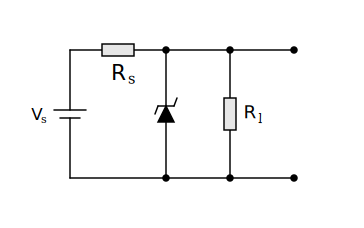
\includegraphics[width=.48\textwidth]{circuit-20231005-2243.png}}
\caption{Simple voltage regulator circuit made from zener diode \label{thcir1}}
\end{figure}

As you can see we have a zener diode parallel to the power supply, which regulates at a certain degree. Since this is a linear circuit output voltage can be easily derived.

Applying kirchhoff current low in the figure \ref{thcir1},


\begin{align*}
I_{z} & = I_{R_s} -I_{L}\\
& = \frac{V_s-V_o}{R_s}-\frac{V_o}{R_L}\\
& = -V_o(\frac{1}{R_s}+\frac{1}{R_L})+ \frac{V_s}{R_s}\\
& = -V_oA^{\prime}+B^{\prime}
\end{align*}

Here, $A^{\prime} = (\frac{1}{R_s}+\frac{1}{R_L})$ and $B^{\prime} = \frac{V_s}{R_s}$.  

We can write $I_z = \frac{V_z}{R_z}$, where $V_z$ and $R_z$ are respectively zener voltages and impedance.  This relation is quite linear in the breakdown region as you can see in the figure \ref{thiv}. \footnote{Image is taken from Electronics Devices and Circuit Theory by Robert Boylsted}

\begin{figure}[hbt!]
\centering{\includegraphics[width=.48\textwidth, trim={.8cm 0.6cm .8cm .5cm},clip]{thzenerIV.png}}
\caption{theoretical current and voltage relation for zener diode \label{thiv}}
\end{figure}


Here we can assume equivalent circuit of \ref{thcir1} as figure \ref{thcir2} 

\begin{figure}[hbt!]
\centering{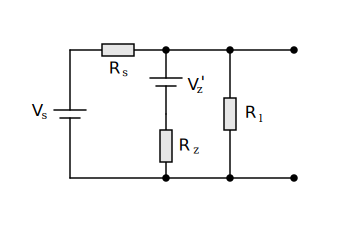
\includegraphics[width=.48\textwidth]{circuit-20231005-2244.png}}
\caption{Equivalent circuit of figure \ref{thcir1} \label{thcir2}}
\end{figure}

Further, simplifying the circuit,

\begin{figure}[hbt!]
\centering{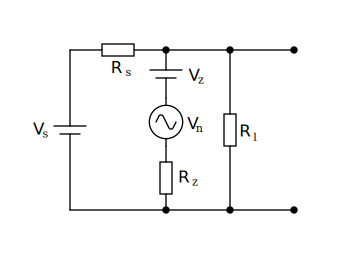
\includegraphics[width=.48\textwidth]{circuit-20231005-2245.png}}
\caption{Equivalent circuit of figure \ref{thcir2} \label{thcir3}}
\end{figure}

This circuit is further simplified as we take $V_z = V_{DC} + V_n$ where $V_n$ is the noise voltage of the zener diode.
If we neglect noise from other sources like resistors and power supply then from figure \ref{thcir3},

\begin{align*}
\frac{V_z}{I_z} & = -V_oA^{\prime} +B^{\prime}\\
\frac{V_{DC}+V_n}{I_z} & =  -V_oA^{\prime} +B^{\prime}\\
V_n & = -V_oA+B
\end{align*}


\begin{align} \label{vo}
V_o & = -\frac{V_n}{A}+\frac{B}{A}
\end{align}



So, we can conclude that here as $V_o \propo V_n$.  This will be the main focus of this project. Here we are neglecting $V_{DC}$ and will be totally okay when we read data from the LOCK IN amplifier, since the DC component has zero frequency which can’t be read from the LOCK IN amplifier.

\subsection{Different noises in the circuit \label{thno}}

The noise voltage $V_n$ is made from different types of noise source which can act as a symbol voltage source. So, $V_n$ can be broken into sub noise sources such as $V_n = V_{flicker}+V_{thermal} + V_{shot} +\cdots$. We will see this noise source and its origin then we will derive its respective distribution and equations.\cite{reggiani1997monte}\cite{wilamowski2018fundamentals}

\begin{figure}[hbt!]
\centering{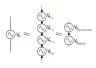
\includegraphics[width=.48\textwidth]{noiseeq.png}}
\caption{Equivalent noise sources}
\end{figure}

\subsubsection{Flicker Noise \label{thflicker}}

Flicker noise is also known as 1/f noise in view of the fact that power density decreases with increasing frequency. This implies that at lower frequencies, the flicker noise dominates.
This type of noise is found  almost in any electronic device which is able to operate at lower frequencies.The main source of this type of noise is D.C supply. Its first evidence was given by J. B. Johnson \cite{johnson1925schottky}. Its first 1/f form is derived by beck and spruit \cite{beck19781}. Now the form is given as 

\begin{align}
S(f) & = \frac{\gamma}{f^{\alpha}}
\end{align}

Here, $\gamma$ and $\alpha$ determine the nature of flicker noise. $\alpha$ determine relations with other noise elements.

\begin{enumerate}
\item ($\alpha > 0$): This means that white noise is dominating the flicker noise as frequency increases.
\item ($\alpha = 0$): This means that only white noise is exists
\item ($\alpha < 0$): This means noise is increasing as frequency. Also, shows that noise will be persistent with a higher range of frequencies. Typically white noise dominates traditional flicker noise.
\end{enumerate}

We can see noise levels as from figure \ref{thnoise}. mostly flicker noise is at considered as $1/f$ noise. In which $\alpha = 1$.

\subsubsection{$1/f^2$ noise}
$1/f^2$ noise is a derivative of  $1/f$ noise and it's mostly seen in metal interconnections of intregrated circuits.

It is modeled by following,
\begin{align*}
  S_{1/f^2}(f) = C \frac{j^{\beta}}{f^{\gamma}\cdot T}\cdot e^{\frac{-E_a}{kT}} 
\end{align*}

Here, C is costant which can be found from experiment, $E_a$ is activation energy for electromigration, $k$ is boltzmann contant, $T$ is temperature. $j$ is current density, $\beta$ and $\gamma$ are contants canbe found from experiment. ($\beta \geq 3$ and $\gamma \geq 2$).
\subsubsection{Shot noise \label{thshot}}

Shot noise is a form of noise that arises because of the discrete nature of the charges carried by charge carriers, electrons or holes or photons hitting the surface. Shot noise is analogous to the rainfall in which raindrop hitting the surface can be considered as discrete. The sound of rainfall is very similar to noise we hear from speakers when we are considering shot noise. Foundational studies in shot noise done my campbell.\cite{campbell1909study}

Since, shot noise is a phenomenon for discrete charge passing through a junction, it can be modelled by poisson distribution. Suppose that In the time interval the $\tau$ Q charge passes through a junction in a semiconductor device (in present context zener diode). This gives rise to discrete probability distribution,

\begin{align}
P(N) & = \frac{e^{-\lambda \tau}(\lambda \tau)^{N}}{N!}
\end{align}

If $N=0$ charge passes in time interval $\tau$ then $P(N)$will be,

\begin{align} \label{eqN0}
P(0) & = e^{-\lambda \tau}
\end{align}

Now suppose, probability of one and only one charge passing through junction in time $\tau$,

\begin{align*}
P(\tau)d\tau & = (P_{\tau}(0))(P_{\tau}(1))
\end{align*}

From equation \ref{thN0},


\begin{align*}
P(\tau)d\tau & = (e^{-I_0 \tau})(e^{-I_0 d\tau} I_0 d\tau)\\
P(\tau) & = (e^{-I_0 (\tau + d\tau)}) I_0
\end{align*}

We can write this equation in frequency domain and by,

\begin{align}\label{thgenl}
P(f) & = S df
\end{align}

Where S is the spectral density of noise.

Here we can write specific form for shot noise in equation \ref{thgen}.\cite{campbell1909study}

%% \cite{campbell}

\begin{align}\label{thshotvo}
\langle V_{shot}^2\rangle & = 2 e I_0 df
\end{align}

Here, $e$ is electron charge,

$I_0$ is average current,

$df$ is ENBW = Equivalent Noise Bandwidth

\begin{align}\label{thshots}
S(f) & = 2 e I_0
\end{align}

\begin{figure}[hbt!]
\label{thnoise}
\centering{\includegraphics[width=.48\textwidth]{thnoise.png}}
\caption{Equivalent noise sources}
\end{figure}

This spectral density gives independence to frequency, which is called white noise. 


\subsubsection{Avalanche or zener noise \label{than}}

avalanche noise often considers the device's operating characteristics in the avalanche breakdown region. It is a major problem where the device is working in avalanche breakdown regions. It is multiplicative noise where chains of electrons crossing from junction rise to noise behaviour. It is very similar to shot noise and we can use that model and just use a multiplicative element in it. In our circuit this is significant since we are dealing with zener diode. With potential gradient inside the zener diode, if any hole and electron pair generates, it gets dragged by potential and hits the other lattice. This creates chain reaction and very high amplitude noise measured.


\begin{align*}
\langle V_{avalanche}^2\rangle & = M \langle V_{shot}^2\rangle
\end{align*}

\begin{align}\label{thavvo}
\langle V_{avalanche}^2\rangle & = 2 e M I_0 df
\end{align}

So, the spectral density $S(f)$ of this noise will be nearly white.
 
Here, we can combine this both avalanche and shot noise to make one noise source,

\begin{align*}
\langle V_{s}^2\rangle & = \langle V_{shot}^2\rangle+\langle V_{avalanche}^2\rangle\\
& = 2 e I_0 df + 2 e M I_0 df\\
& = (M+1) 2 e I_0 df\\
\end{align*}

And spectral density will be $S(f) = (M+1) 2 e I_0$

Since this noise is white noise we can measure at every frequency. This is what we are going to do in the next chapter.



\subsubsection{Thermal noise \label{thth}}

Thermal noise, also called Johnson–Nyquist noise is the electronic noise generated by random motion of charge carriers. This charge carrier is generated by the thermal agitation inside an electrical conductor at equilibrium, which happens regardless of any applied voltage. Because of their random motion it can be said that they have a mean value at zero. This reason says that we can't model this noise by poisson distribution but have to model with normal or gaussian distribution. In 1936, J B Johnson first gave an idea about thermal noise in thermionic valves. \cite{johnson1928thermal}

The noise amplitude is very similar to that of shot noise and given as,

\begin{align}\label{ththvo}
\langle V_{thermal}^2\rangle & = 4 K_B R df
\end{align}

Here, $K_B$ is boltzmann constant,

R is resistance of device or component,

$df$ is ENBW.

\begin{align*}
S(f) & = 4 K_B R
\end{align*}


By equation \ref{thths} we can see that thermal noise in an ideal resistor is approximately white, meaning that the power spectral density is nearly constant throughout the frequency spectrum. But practically it does decay to zero at extremely high frequencies (terahertz for room temperature). Also, we are neglecting quantum effects. 


Total noise in the circuit will bre frequency dependent noise and white noise,


\begin{align*}
V_n & = V_{n}(f)+ V_{white}\\
S(f) & = \frac{\gamma}{f^{\alpha}}+(2e(M+1)I_0+4K_bR)+\mathcal{O}(other)
\end{align*}

\begin{align}\label{theoryvn}
S(f) & \approx \frac{\gamma}{f^{\alpha}}+(2e(M+1)I_0+4K_bR)
\end{align}

which is main derivation of our project.


\section{Methodology}\label{methodology}

\subsection{Our voltage regulation circuit}

Our purpose was to regulate voltages and also study noise related to the circuit. If we choose a complicated circuit for voltage voltage regulation then analysis of noise will be relatively complicated. So, we used a very basic voltage regulator circuit from a zener diode. Supply was given as DC power supply with voltage $V_{s}$. This voltage is decided by the zener voltage at hand.

The noise in the circuit will be relatively higher at the zener breakdown region. As we discussed from the theoretical part, noise power will be proportional to current flowing in the zener diode (here, we are assuming that noise from other parts is almost zero). To prepare a zener diode (BZX55C5V1) to break down the region we choose 5.4V. This is calculated from 
For our purpose we utilised a general purpose zener diode with breakdown region between 4.8V to 5.4V with current of $\mu A$ order. We first did the Current and voltage characteristics of zener diodes. The useful information we got from there is source voltages, zener voltages and current that we particularly needed in our project. Our aim was to never exceed the LOCK IN amplifier’s input limits. Current and voltage characteristics are down in figure \ref{exiv}. The zener diode we used had its datasheets, which you can see from Appendix. Its power rating is … 

\begin{figure}[hbt!]
\centering{\centering\includegraphics[width=.48\textwidth]{zener.png}}
\caption{Our zener diode}
\end{figure}

The zener diode was given proper voltages to work in reverse bias, specifically in the breakdown region. The overall circuit was identical to that of voltage regulator by zener diode. We gave particularly 5.0 V, 5.5V in two different runs from the powersource. The Zener diode regulated around 4.9 V. 

\begin{figure*}[hbt!]
\centering{\centering\includegraphics[width=1\textwidth]{zenerIV.png}}
\caption{current and voltage characterists of zener diode \label{exiv}}
\end{figure*}

Now, what we need is that fluctuation over the regulated DC voltage. These fluctuations have to be some function in the frequency domain as we assumed. This function must be made of different harmonics of sinusoidal waves with different phases and frequencies as thought by Fourier and his analysis. So basically we needed a system to measure different amplitudes of these harmonics at different frequencies to model our fluctuations. We needed a complete frequency spectrum at the particular bandwidth we are looking for in this analysis. The LOCK IN amplifier gives exactly that. 


\subsection{Measuring instrument: LOCK IN amplifier}

LOCK IN amplifiers came in the 1930s and became very important in signal extraction from given frequency and phase. It is very helpful in measuring signals in a very noisy environment. It takes two inputs, one which is being measured and one which is given as a reference mono frequency signal. Reference signal gets multiplied with input signal and gives output through a process called Phase sensitive detection in which it uses homodyne detection scheme and filters out signal as DC component. We will see in a bit.

\subsubsection{Phase sensitive detection}

In nutshell it uses frequency multiplication and generates double side bands which then pass through a low pass filter to extract signal. In figure \ref{psd} you can see a signal first goes into a low noise differential amplifier which strengthens the signal. Signal Gets multiplied by another reference signal. This gives rise to two bands which pass through a low pass filter which cancels higher degree signal and only left is low frequency signal.


\begin{figure}[hbt!]
\centering{\centering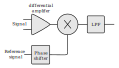
\includegraphics[width=.48\textwidth]{PSD.png}}
\caption{basic phase sensitive detector}
\end{figure}

If we take signal $V_s(t)$ with frequency $w_s$, amplitude $A$ and phase $\theta$. 

\begin{align*}
V_{s}(t) & = A \cos(w_st+\theta)\\
\\
& = \frac{A}{2} (e^{i(w_st+\theta)}+e^{-i(w_st+\theta)})\\
\end{align*}

Reference signal can be taken as following,

\begin{align*}
V_r(t) & = B (e^{-i(w_rt+\phi)})
\end{align*}

In common settings, $\phi = 0$ and $B=1$,

\begin{align*}
V_r(t) & = e^{i(-w_rt)}
\end{align*}

Together after mixing the signals we have,

\begin{align*}
Z(t) & = V_s(t)\timesV_r(t)\\
\\
& = \frac{A}{2}(e^{i\left[ (w_s-w_r)t+\theta \right]}+e^{-i\left[ (w_s+w_r)t+\theta \right]})\\
\\
& = X(t)+Y(t)
\end{align*}

Making $w_s=w_r$ which makes subtraction vanishes and only one term with higher frequency lefts. Passing this signal through a low pass filter with very low cutoff gives only DC components and rejects noise even from neighbouring frequencies.


\begin{align*}
Z(t) & = \frac{A}{2}(e^{i \theta})
\end{align*}

Two component $X(t)$ and $Y(t)$ becomes,

\begin{align*}
X(t) & =\re(Z(t))\\
\\
& =  \frac{A}{2}\cos(\theta)
\end{align*}

And,

\begin{align*}
Y(t) & = \im(Z(t))\\
\\
& =  \frac{A}{2}\sin(\theta)
\end{align*}

So, Amplitude and Phase becomes, 

\begin{align*}
R & = \sqrt{X(t)^2+Y(t)^2}\\
\\
& =  \sqrt{(\frac{A}{2}\cos(\theta))^2+(\frac{A}{2}\sin(\theta))^2}\\
\\
& = \frac{A}{2}\\
\\
\Theta & = \arctan(\frac{Y}{X})
\end{align*}

So, the final product in PSD is the absolute amplitude of the signal and its phase. 

\subsubsection{Time Constant }

\subsubsection{ENBW}

\subsubsection{Sensitivity} 

\subsubsection{LOCK IN amplifier over traditional measuring device/system}

For noise analysis LOCK IN amplifiers are the optimal choice. Traditional approaches deal with the first measurement of a small signal in the time domain. This signal gets amplified with additional noise from the amplifier. Also, amplifiers attenuates signals with its limited bandwidth which is a measure of concern for certain use case scenarios. This attenuated signal gets into some detector. For signal analysis, this signal must go into other  processes like analog to digital conversion then Fourier transformation. This whole process gives too much concerned noise which is not related to devices being analysed in our case the voltage regulator circuit. Alternative approach is to go with a LOCK IN amplifier. Which cancels out most burdens of traditional measurement steps. This whole combined help in reducing internal noise and increasing S/N ratio.
\\
\\
\emph{\large Pros of LOCK IN amplifier:}
\begin{itemize}
\item LOCK In amplifiers reduces attenuation of signal with increasing frequency since it does not measure signal in the whole frequency spectrum.
\item Increase S/N ratio over traditional amplifier circuit
\item Gives direct data into frequency domain
\end{itemize}\\
\\
\emph {\large Cons of LOCK IN amplifier:}
\begin{itemize}
\item Relatively expensive
\item Does not give information in time domain
\item Relatively slow for whole analysis of frequency domain (low but accurate resolution of frequency domain)
\end{itemize}

\subsection{SR830}

We used a LOCK IN amplifier from Stanford Research Systems. It is used to detect low amplitude signals as low as $10\frac{nV}{Hz}$ and frequency as low as $100mV$.  and measure very small AC signals - upto few nanovolts. Accurate measurements may be made even when the small signal is obscured by noise sources many thousands of times larger.


Internal block diagram of SR830,

%% \begin{figure*}[hbt!]
%% \centering{\centering\includegraphics[width=.55\textwidth,page=33,trim={5cm 5cm 5cm 10cm, clip}]{sr830m.pdf}}
%% \end{figure*}

\subsubsection{Inputs}

\subsubsection{Outputs}

\subsubsection{Interfacing}



Lock-in amplifiers use a technique known as
phase-sensitive detection to single out the component of the signal at a specific reference frequency and phase. Noise signals at frequencies other than the reference frequency are rejected and do not affect the measurements.


Now , on the basis of frequencies/ frequency levels and its origin, there are different types of noises are present in our environment. Some of them are discussed below:


\section{Results and Analysis}

We have surveyed voltage regulated circuits we made with zener diodes and found some satisfactory results. We take different results for different bandwidths. For context this is row data from different bandwidth. Here, for each set of frequencies in bandwidth we took almost 50 to 100 readings.


\subsection{Low frequency: up to 10k hertz}

We are mainly focused low frequency results since we are only intrested in regulated power supply applications. We had original assumption that in low frequency flicker noise is higly dominating.

\begin{figure}[hbt!]
\centering{\includegraphics[width=.5\textwidth,trim={.5cm 0cm 1cm 0cm}, clip]{raw_1000_100us.png}}
\caption{This is row data for 1k to 10k frequency band TIME CONSTANT = $100\mu s$ and $12dB/oct$}
\end{figure}\\

Here initial results were quite random, which means we have to filter our data a bit. For this reason we used a basic filtering method. In this method the data are sorted out as minimum deviation from their minimum then we took the upper 5 to 10 results and took the mean of it. The basic implementation is as following,

Let, $X(f)$ as data point for specific $f$ and $Y(f)$ be sorted data with $n$ number of results,
\begin{align*}
\langle X(f) \rangle & = \sum_{i=0}^{N-1} X^{(i)}(f)\\
Y_n(f) & = min(t\: such\: that\: \# \{ s =\\
&   \lvert X(f)- \langle X(f)\rangle \rvert \;| s \geq t \} =n)\\
\langle Y(f) \rangle & = \sum_{i=0}^{n} Y^{(i)}(f)
\end{align*}

This is how we implemented it with python. If you wanna checkout whole code then it is in the appendix.

\begin{minted}[%
breaklines,    
breakanywhere,
mathescape,
xleftmargin=20pt,
linenos]{python}
for datapoint in data:
    count+=1
    if datapoint[0]==index:
        temp_erray.append(float(datapoint[1]))
    else:
        nlist = array(temp_erray,dtype=float)
        m = mean(nlist)
        sorted_deviation = argsort(abs(nlist - m))
        filtered_nlist = nlist[sorted_deviation[:points]]
        indexonelist = array([index]*points)
        final_list= column_stack((indexonelist,filtered_nlist))

\end{minted}

Also, as discussed from the previous section we have to correct these terms with ENBW. Time constant (T)= 100$\mus$ and roll-off =12 $dB/oct$
       
\[
ENBW = \frac{1}{8T} = 1250 Hz 
\]



\begin{figure}[hbt!]
\centering{\includegraphics[width=.5\textwidth]{final_1000_100us.png}}
\caption{final analysed data for 1k to 10k hertz frequency with TIME CONSTANT = $100\mu s$ and $12dB/oct$}
\end{figure}\\
 
Here we can see some traces of flicker noise. Parameterized as follows,


\begin{align*}
S(f) & = \frac{\gamma}{f^{\alpha}}
\end{align*}

Here, $\gamma$ and $\alpha$ determine the nature of flicker noise. Results are from theoritical section.

\begin{align}\label{eq1}
S_{flicker}(f) & = 5.90923491 \frac{1}{f^{1.34677368}}\\
S_{white}(f) & =2.0644381e-05
\end{align}


\subsection{Very low frequency: upto 1 hertz}

Let's take a second data set where we have sub hertz frequency data. This data set have each frequency with corresponding 50 values. Raw data looks like figure \ref{rawsubhz}.


\begin{figure}[hbt!]
\centering{\includegraphics[width=.5\textwidth]{raw_1_100us.png}}
\caption{This is row data for sub one hertz band with TIME CONSTANT = $100ms$ and roll of factor $12dB/oct$} 
\label{rawsubhz}
\end{figure}\\


For analysing data ENBW is calculated for TIME CONSTANT = $100ms$ and roll of factor $12dB/oct$},

       
\[
ENBW = \frac{1}{8T} = 1.25 Hz 
\]

Final data will be look like this,

\begin{figure}[hbt!]
\centering{\includegraphics[width=.5\textwidth]{final_1_100ms.png}}
\caption{final analysed data for sub one hertz band with TIME CONSTANT = $100ms$ and roll of factor $12dB/oct$}
\end{figure}\\


Here data feeted at negative $-alpha$,

\begin{align}\label{eq2}
S_{flicker}(f) & =  \frac{-0.64836618}{f^{-0.64836618}}
\end{align}

Here two things is important $\alpha < 0$ and $\gamma$ is small.

\subsection{High frequency data: up to 100k hertz}

Same as we discussed previously raw data is given here, we have up to 50khz frequency domaoin data,


\begin{figure}[hbt!]
\centering{\includegraphics[width=.5\textwidth]{raw10000100ms.png}}
\caption{This is row data for high frequency band with TIME CONSTANT = $100ms$ and roll of factor $12dB/oct$} 
\label{raw100k}
\end{figure}\\

same as previous sections, we sorted data and take ENBW calculations at here.

\begin{figure}[hbt!]
\centering{\includegraphics[width=.5\textwidth]{final_10000_100ms.png}}
\caption{final analysed data for high frequency band with TIME CONSTANT = $100ms$ and roll of factor $12dB/oct$}
\end{figure}\\

the noise spectral density is as following.

\begin{align}\label{eq3}
S_{flicker}(f) & = \frac{0.13707877}{f^{0.92287006}}\\
S_{white}(f) & = 1.20525914e-05
\end{align}


Here this parameters are similar to that of first data set aka low frequency data.

\section{Conclutions}

In 1k to 10k data, we have specified flicker noise power AKA $(\frac{1}{f})^{\alpha}$ as $\alpha = 1.34677368$, which is close to flicker noise theoretical values for maximum flicker noise which is equal to 1. white noise level in $\mu V$ region, which is expected (at $2.0644381e-05$). 


The most mysterious results came from second data sets, very low frequency data sets. Here  $\alpha= -0.64836618$ which is negative. This means that noise increases as frequency increases, this case already discussed in theoritical part. Our assumtion here is that as frequency increases the white noise gets saturated to it’s related power. This means that white noise is not quite white as it seems. Assumption is also be made that frequency dependence of flicker noise is not quite like that of distrubution as theory discussed. Well, we have to dig deep into that.

Last data set is quite normal, it satisfy first data sets and closely correlate with the theoritical model. We have white noise level is similar to that of first data sets with different is of $2.0644381e-05-1.20525914e-05 = 0.85917896e-05$. which is very small. 

Further studies can be conducted to anamolous behaviour at very low frequency noise $\approx 1Hz$. This can be important in regulated power supply usage since 1Hz is very near to DC level. 

We hope that our contribution to Open source community is well recevied and gets more contribution to our package \textbf{PyInstro}.




\addcontentsline{toc}{section}{References}
\bibliographystyle{plain}
\bibliography{documentation}

\onecolumn



\addcontentsline{toc}{section}{Appendix}
\addcontentsline{toc}{subsection}{PyInstro}
\addcontentsline{toc}{subsection}{Code for data analysis}
\addcontentsline{toc}{subsection}{Zener diode datasheet}
\section*{Appendix}

\subsection*{PyInstro}

PyInstro is a package we made to communicate, control and data logging to any scientific instrument easily. The main work of it is giving utility for data logging and ease SCPI. Also, it does streamline instruments after extending it. It is just a cover for the PYVISA backend but it gives instrument specific tools. whole package in the following link,
This is code for just the GPIB connection which we used. (it is also extensible to the RS232, LAN and USB )

%% \begin{table*}[hbt!]
\emph{GPIB.py}
\begin{minted}{python}
import pyvisa
import sys
from termcolor import cprint

class GPIB:
    def __init__(self) -> None:                                 
        try:                        # GPIB connection check
            cprint("-----------checking GPIB connections--------",color="yellow")
            resources = pyvisa.ResourceManager()
            interface = None
            resourceslist = resources.list_resources()
            cprint(resourceslist,'blue',attrs=['bold'])
            if resourceslist==():
                cprint("ERROR: please check GPIB connection", "red")
                sys.exit()
            else:
                while True:
                    try:
                        choise = int(input("please, choose your device from this list: "))-1
                        if choise>len(resourceslist):
                            TypeError
                        interface = resourceslist[choise]
                        cprint("-------------chose resource-----------------",color="green",attrs=["bold"])
                        cprint("-------following device is connected--------",color="green",attrs=["bold"])
                        cprint(interface)
                        break
                    except:
                        cprint("choose with interger and from following...","red")

            self.interface =  resources.open_resource(interface)
        except:
            cprint("ERROR in detecting GPIB, there must be problem with setup of pyvisa or there is no connection of gpib\n you should look either in pyvisa documentation or try for RS232 interface","red",attrs=['bold'])
            sys.exit()

    def ping(self)-> None:
        self.interface.write("*IDN?\n")

    def read(self)-> None:
        self.interface.read()

    def reset(self)-> None:
        self.interface.write("*RST\n")

    def clear_status(self)-> None:
        self.interface.write("*CLS\n")

    def close(self)->None:
        self.interface.close()

    def std_event(self)->None:
        pass

\end{minted}
%% \end{table*}

This is SR830 device commands,

\emph{SR830.py}
\begin{minted}{python}
from pyinstro.utils import sysarg
from pyinstro.utils import datafile

new_instance = sysarg.CLI()

if new_instance.get_connection()=="GPIB":
    from pyinstro.interfaces import gpib
    
    class SR830(gpib.GPIB):
        def __init__(self) -> None:
            super().__init__()

            file_init = datafile.Get_File(new_instance.get_file())
            
            self.get_levels = new_instance.get_levels
            self.get_partitions = new_instance.get_partitions
            self.writerow = file_init.writerow
            self.longwriterow = file_init.longwriterow
            self.fmin = new_instance.get_fmin
            self.fmax = new_instance.get_fmax
            self.freq = new_instance.get_freq

        def local_defaults(self)-> None:
            pass

        def local_arguments(self)-> None:
            new_instance.argparser.add_argument('-fl','--fmin', metavar='', type=float, default=4545, help="give lower limit for reference frequency")
            new_instance.argparser.add_argument('-fr','--freq', metavar='', type=float, default=7888, help="give reference frequency")
            new_instance.argparser.add_argument('-fh','--fmax', metavar='', type=float, default=1, help="give upper limit for reference frequency")
    
        def set_frequency(self, value, errdelay = 3) -> None:
            """change reference frequency"""
            self.interface.write("FREQ "+"{:.4E}".format(value))
            pass

        def autogain(self)->None:
            self.interface.write("AGAN")

        def set_phase(self,value) -> None:
            self.interface.write("PHAS "+str(value))
            pass

        def time_constant(self,choise) -> None:
            self.interface.write("OFLT "+str(choise))
            pass

        def sensitivity(self,choise) -> None:
            self.interface.write("SENS "+str(choise))
            pass

        def set_sample_rate(self, choise)->None:
            self.interface.write("SRAT "+str(choise))

        def start_data_acquision(self) -> None:
            self.interface.write("STRT")
            pass

        def pause_data_acquision(self) -> None:
            self.interface.write("PAUS")
            pass

        def reset_data_acquision(self) -> None:
            self.interface.write("REST")
            pass

        def get_data(self) -> None:
            pass

        def get_data_explicitly(self, data_variable=3, errdelay=3):
            """
            two params, give resource object and the second params is parameter to variable read,
            default to data_variable = 3 which is equievalent to reading R.
            as SR830manual, 
            data_variable = 1 => X,
            data_variable = 2 => Y,
            data_variable = 3 => R,
            data_variable = 4 => phase
            """
            return self.interface.query("OUTP? "+str(data_variable))

        
else:

    from pyinstro.interfaces import rs232
    
    class SR830(rs232.RS232):
\end{minted}

This is some utilities to ease control of scientific instruments,

FIlewrite \ simple data logger: \emph{getfile.py}

\begin{minted}{python}
from pyinstro.utils import getpath



import csv
import os



class Get_File:
    """
    INFO: just to write file, must be CSV 
    """
    def __init__(self,file) -> None:
        _project_dir_path_abs = getpath.getpath()

        if os.path.exists(os.path.join(_project_dir_path_abs,"data")):
            _data_dir_path_abs = os.path.join(_project_dir_path_abs,"data")
        else:
            os.mkdir(os.path.join(_project_dir_path_abs,"data"))
            _data_dir_path_abs = os.path.join(_project_dir_path_abs,"data")
        
        if file=='default':
            file = "auto0.csv"
            count = 0
            while os.path.exists(os.path.join(_data_dir_path_abs,f"auto{count}.csv")):
                count+=1
                file = f"auto{count}.csv"

        file = os.path.join(_data_dir_path_abs,file)
        
        # i did not used re module down here
        if not ((file[len(file)-1]=='v')and(file[len(file)-2]=='s')and(file[len(file)-3]=='c')and(file[len(file)-4]=='.')):
            file = file+".csv"
        else:
            pass
        
        self.filepath = file
        self.firsttime = True

    def writerow(self, data)-> None:
        """
        open file one time ad write it
        """
        if self.firsttime:
            self.file = open(self.filepath,'w',newline='')
            self.writer = csv.writer(self.file)
            self.writer.writerow(data)
            self.firsttime = False
            print(self.filepath)
        else:
            self.writer.writerow(data)


    def longwriterow(self,data)->None:
        """
        for long data, i think it is suitable to write file each time open and close
        """
        with open(self.filepath,'a',newline="") as datafile:
            self.writer = csv.writer(datafile)
            self.writer.writerow(data)

\end{minted}


DEFAULT setting: \emph{defaults.py}

\begin{minted}{python}
from pyinstro.utils import getpath

import os
import configparser

class DefaultParams:
    """
    specify default parameters
    
    for more info:
    refer to SR830 manual for more info.
    """
    time_constant = 5
    sensitivity = 5
    # filter_slope = 

    baud_rate = 9600
    sample_rate = 10
    gpib_address = 1
    time_delay = 1

    connection = 1          # means GPIB, 1: GPIB, 2: RS232, 3: USB, 4: LAN
    connections = {1:"GPIB", 2:"RS232", 3:"USB", 4:"LAN"}

    fmin = 01E+3
    fmax = 01E+5
    
    partitions = 4
    levels = 4

    data= 3

    def __init__(self) -> None:
        self.defaults_params_list= [attr for attr in dir(self) if not callable(getattr(self, attr)) and not attr.startswith("__")]
        #defaults_params= dict(zip(defaults_params_list,list(" "*len(defaults_params_list))))
        
        self.target_path = getpath.getpath()
        config_file = os.path.join(self.target_path,"config.ini")

        print("checking config.ini file")
        
        if os.path.exists(config_file):
            config = configparser.ConfigParser()
            config.read(config_file)
            config_file_dict = config.defaults()
            if len(config_file_dict)==len(self.defaults_params_list):
                for keys in config_file_dict:
                    if (config_file_dict[keys].isspace() or not config_file_dict[keys]):
                        pass
                    else:
                        setattr(self, keys, config_file_dict[keys])
                        print(keys+":  "+config_file_dict[keys])
            else:
                for keys in self.defaults_params_list:
                    if not (keys in config_file_dict):
                        with open(config_file, "w") as _conf_file: 
                            config.set("DEFAULT",keys," ")
                            config.write(_conf_file) 
                    else:
                        if (config_file_dict[keys].isspace() or config_file_dict[keys] ==""):
                            pass
                        else:
                            setattr(self, keys, config_file_dict[keys])
                            print(keys+":  "+config_file_dict[keys])
                            
        else:
            pass

    def makeconfig(self):
        config_file =os.path.join(self.target_path,"config.ini")
        config = configparser.ConfigParser()
        if os.path.exists(config_file):
            config.read(config_file)
            config_file_dict = config.defaults()
            if len(config_file_dict)==len(self.defaults_params_list):
                pass
            else:
                for keys in self.defaults_params_list:
                    if not (keys in config_file_dict):
                        with open(config_file, "w") as _conf_file: 
                            config.set("DEFAULT",keys," ")
                            config.write(_conf_file)
                            
                    else:
                        pass
                print("I had appened to full option to config file!")
        else:
            with open(config_file,'w') as config_file:
                config_file.write("[DEFAULT]\n")
                for params in self.defaults_params_list:
                    config_file.write(params+" = \n")
            print("I had made config file in present directory !")

\end{minted}

            

\subsection*{Code for data analysis}
\input{analysis}
\clearpage
\subsection*{Zener diode datasheet}
\begin{figure*}[hbt!]
\centering{\centering\includegraphics[width=.55\textwidth,page=1,trim={1cm 1cm 1cm 1cm, clip}]{sr830m.pdf}}
\end{figure*}
\clearpage
\begin{figure*}[hbt!]
\centering{\centering\includegraphics[width=.55\textwidth,page=2,trim={1cm 1cm 1cm 1cm, clip}]{sr830m.pdf}}
\end{figure*}
\end{document}


